\chapter {Mechanism of orientation selectivity in the tree shrew V1}
\pagebreak
\section{Summary}
\pagebreak
\section{Introduction}

Cortical units selectively respond to edges of a narrow range of orientations unlike their Lateral Geniculate Nucleus (LGN) counterparts which respond well to most orientations. Hubel and Wiesel proposed that this orientation selectivity came from un-oriented, spatially offset LGN receptive fields arranged collinearly along the long axis of the cortical neuron to which they provide input (Hubel \& Wiesel, 1962; 1968). While this model explains certain features like length summation in the cortical neurons, it is unable to account for the contrast invariance reported in simple cells (Sclar \& Freeman, 1982), the role of intracortical inhibition in sharpening orientation selectivity (Creutzfeldt et al., 1974; Sillito, 1975; 1979; Tsumoto et al., 1979; Sillito et al., 1980) and the presence of orientation biases in the LGN neurons (Vidyasagar \& Urbas, 1982; Smith et al., 1990). In the light of these short comings, alternate models of orientation selectivity have been proposed.

Other models of orientation selectivity in V1 include cross-orientation inhibition (Creutzfeldt et al., 1974), iso-orientation facilitation (Douglas et al., 1991; Volgushev et al., 1995), spatially offset excitatory and inhibitory inputs (Heggelund, 1981) and excitatory inputs originating from on and off centred neurons (Soodak et al., 1987; Kremkow et al., 2016). The cross orientation inhibition model suggested that V1 neurons receive inhibitory inputs from cortical interneurons which then lead to the sharpening of orientation selectivity (eg: Creutzfeldt et al., 1974; Morrone et al., 1982; Eysel et al., 1990). However, intracellular experiments have shown that both cortical excitation and inhibition tend to be of the same orientation (Ferster, 1986; Anderson et al., 2000). Further, there was no clear explanation for how the inhibitory neurons themselves became orientation selective. The iso-orientation excitation model also suffered from a similar problem. Models where the juxtaposition of on and off sub-regions have been implicated as the origin of orientation selectivity (Soodak et al., 1987; Kremkow et al., 2016) ignore studies where intravitreal application of APB (suppresses ON responses in bipolar cells) did not affect the orientation of the remaining off response (Schiller, 1982, 1986; Sherk \& Horton, 1984; for review see Schiller, 1992).

One model of orientation selectivity suggested that the basis of orientation selectivity was already established in the sub-cortical regions. In this model, cortical neurons get weakly oriented inputs which are then sharpened by intracortical mechanisms (Vidyasagar, 1987; Somers et al., 1995; Vidyasagar et al., 1996; Vidyasagar \& Kuhlmann, 2011; Vidyasagar \& Eysel, 2015).  Orientation biases have been demonstrated in the retina and LGN of  (Vidyasagar \& Urbas, 1982; Naito et al., 2013), macaques (Shou \& Leventhal, 1989; Smith et al., 1990) and tree shrews (Van Hooser et al., 2013). This model successfully explains contrast invariance in V1 neurons (Naito et al., 2013; Viswanathan et al., 2015) and length tuning (references). It also gives a way through which orientation selectivity of inhibitory inputs are established and does not rely on the relative positions of the on and off inputs to establish orientation selectivity.

A mechanism through which sharp orientation selectivity in V1 may be generated from biased geniculate inputs is elaborated below. When studied using sine-wave gratings of varying spatial frequencies, cortical cells exhibit band-pass spatial frequency tuning i.e., they responded to a narrow range of spatial frequencies. Their LGN counterparts on the other hand showed low-pass spatial frequency tuning (Maffei \& Fiorentini, 1973; DeValois et al., 1980; Van Hooser et al.,2013). When the orientation of the grating was also varied, at lower spatial frequencies, retinal and LGN neurons respond well to gratings of all orientations. At higher spatial frequencies, on the other hand, the orientation selectivity sharpens markedly; i.e., the response at the non-optimum orientation was less when compared to the optimum orientation (Levick \& Thibos, 1980; 1982; Vidyasagar \& Heide, 1984; Naito et al., 2013). Most cortical neurons received mono-synaptic excitatory inputs and disynaptic inhibitory inputs from LGN neurons (Reference). At lower spatial frequencies, the orientation non-specific inhibition from the geniculate inputs attenuates the spatial frequency response of the cortical neurons via inhibitory interneurons, making them band-pass tuned to spatial frequency (Vidyasagar \& Heide, 1984; Bredfeldt \& Ringach, 2002). At the higher spatial frequencies where both the cortical and the LGN neurons respond, the LGN neurons demonstrates sharp orientation tuning (Vidyasagar \& Heide, 1984l Vidyasagar, 1987; Kuhlmann \& Vidyasagar, 2011). It has been showed that given the same eccentricity, the highest spatial frequencies for which the LGN neuron responds is not significantly different from the peak spatial frequency of the layer 4 neurons (Naito et al., 2013). The layer 4 neurons in cats could therefore get their orientation selectivity from LGN neurons that show sharp orientation tuning at higher spatial frequencies. Here we wanted to examine if a similar mechanism is in place in the Tree Shrews. 

The tree shrew is a highly visual, diurnal mammal that is closely related to primates. The tree shrew V1 is organized in layers, with layer 4 segregated into on and off sub-regions (Conley et al., 1984; Kretz et al., 1986). The layer 4 of tree shrew V1 retains LGN like receptive field properties and it has been suggested that the transformation of RFs that occurs from the LGN to layer 4 in cats occurs from layer 4 to layer 2/3 in tree shrews (Chisum et al., 2003; Mooser et al., 2004; Lee et al., 2016 ). Given that matched recordings from LGN and V1 are fairly difficult to perform, the tree shrew provides an opportunity to examine the transformation of orientation selectivity in a single electrode penetration. This also gives the added advantage of recording from neurons that are matched for eccentricity, as this is an important caveat while recording spatial frequency tuning from different visual areas.

In the tree shrew, orientation selectivity in layer 2/3 neurons is said to come from excitatory convergence of a number of layer 4 neurons (Mooser et al., 2004) with the horizontal connections further sharpening the orientation selectivity (Bosking et al., 1997; Chisum et al., 2003; Mooser et al., 2004; Veit et al., 2013). One study that used optogenetics and optical imaging of intrinsic signals showed that horizontal connections in the layer 2/3 of tree shrew V1 did not have a modulatory effect on the neuronal responses as expected (Huang et al., 2014). However, it must be noted that the optogenetic stimulation would not have activated GABA-ergic neurons in the cortex and any excitation of inhibitory neurons would be post-synaptic which may not have been sufficient to alter the response. Recently, Lee et al. (2016), suggested that orientation selectivity in the shrew V1 was established by on inputs organising themselves around off inputs as has been proposed in cats (Kremkow et al., 2016). However, Muly and Fitzpatrick (1992) showed that on and off inputs to layer 2/3 cells have significant overlap, preventing extensive segregation of the sub-regions. Further, only a small proportion of all cells in the shrew V1 had segregated receptive field sub-divisions (Veit et al., 2013; Van Hooser et al., 2013), lacking the basic RF structure for the majority of the cells to develop orientation selectivity using this method.As a result, the mechanism through which orientation tuning comes about in the shrew V1 is as yet unclear.

It could be that, the orientation selectivity of the layer 2/3 neurons in the shrew V1 could come about by the mechanism proposed by Vidyasagar et al. (1996). It has already been shown that layer 4 neurons in tree shrews show some degree of orientation tuning and low pass spatial frequency tuning responses similar to their LGN counterparts (Humphrey \& Norton, 1980; Chisum et al., 2003; Van Hooser et al., 2013; Scholl et al., 2013). There are extensive short and long range horizontal connections within the tree shrew layer 2/3 which could provide orientation non-specific inhibition to layer 2/3 neurons (Bosking et al., 1997; Chisum et al., 2003). In this chapter, we aimed to further examine the relationship between orientation selectivity and spatial frequency tuning of tree shrew V1 neurons in order to see whether the sharp orientation selectivity seen in the layer 2/3 neurons comes from sharpening the orientation biases established in layer 4. We hypothesised that-


\noindent{\textbf{[H1]}: The Layer 4 neuron will be tuned to the same orientation as the layer 2/3 neuron.}

\noindent{\textbf{[H2]}: The Layer 4 neurons in the tree shrews will be more selective to orientation at higher spatial frequencies.}

\noindent{\textbf{[H3]}: Layer 2/3 neurons will fire optimally where the orientation selectivity of the layer 4 neuron is maximum.
}

\section{Methods}


\subsubsection{Surgery and Anaesthesia}

The following surgical procedures were performed on the tree shrews from whom data were collected for chapters 5 and 6. Surgical procedures are as outlined in the Methods chapter. Briefly, the animal was anaesthetized using a mixture of Ketamine and Xylazine, a venous catheter was inserted in to the femoral vein and a tracheostomy performed to assist in breathing during the experiment. The animal was administered muscle paralysant (Vecuronium Bromide) intravenously and was anaesthetised using Isoflurane (0.5-1\%) for the duration of the experiment. Hard contact lenses were fitted to the eye to prevent corneal drying. In some tree shrews, additional lenses were used to correct for any refractive errors. A craniotomy and durotomy were performed over the location of V1 (Horsley-Clarke Co-ordinates A2.5 to P2.5). ECG and frontal EEG were monitored during the experiment. At the end of the experiment, the animal was euthanized using an overdose of pentobarbital sodium and perfused using 0.1M Phosphate Buffer (PB) solution followed by 4\% Paraformaldehyde in 0.1M PB. The brain was removed and stored in sucrose (20-25\%) for histology.

	\subsubsection{Electrophysiology}
High impedence, lacquer coated tungsten microelectrodes (FHC Metal Microelectrodes Inc., ME, USA; impedance= 12-18 MΩ) were lowered into the brain at an angle perpendicular to the cortical surface. The signal was amplified and filtered (x 10,000 gain, bandpass filtered between 300-3000 Hz, A-M systems) and fed into an audio speaker as well as an analog to digital converter (Cambridge Electronic Design Limited, Cambridge, UK; digitised at 22.5 kHz). Neurons were recorded from Layers 2/3 and Layer 4. Layer 4 could be identified by a characteristic ‘swish’, first for on stimuli and then for off stimuli, in the tree shrews. Where we no longer heard the swish, we concluded that we exited layer 4 and into layer 5. Neurons in layers 5 and 6 were not recorded from. Lesions (6 μA for 6s) were made at the end of each track. The electrode was withdrawn and lesions were made at regular intervals to trace the path of the electrode through the brain. The data was recorded as a spike trace using the spike 2 software (CED, Cambridge, UK). The spikes were templated and the spike timing exported as a text file. Further analysis was performed using custom MATLAB$^{\textregistered\\}$ code (The Mathworks Inc, USA).
\subsubsection{Stimuli}
A hand-held projectoscope was used to mark the receptive field boundaries. Using this, the centre of the monitor was aligned with centre of the receptive field prior to stimulus presentation. Stimuli were presented using a BARCO monitor (Frame Refresh Rate= 80 Hz; Reference Calibrator Plus; Barco Video and Communications, Belgium) and generated using Visage (VSG, Cambridge Research Systems, Cambridge, UK) and custom Stimulus Description Language (SDL) scripts. The monitor had a mean luminance of 32.6 cdm-2. While recording, the monitor was placed at a distance of 114 cm from the eye. For each of the different stimuli described below, ten complete stimulus presentations were completed.
\paragraph{Bar Stimuli}
For each neurons, an initial estimate of optimum orientation was obtained using bars, moving bi-directionally across the screen. The background was a uniform gray screen. Depending on the polarity of the neurons, either a bright bar or a dark bar was used (contrast= 100 \%). The bar was usually 8$^o$o long (ranging between 4 and 8 degrees) and 0.5$^o$ wide (ranging between 0.1 and 1 degree). A total of 18 different orientations were tested and PSTHs (see chapter 2) were made online using the Spike 2 software. The orientation that yielded the highest firing rate was used for further testing.

\paragraph{Grating Stimuli}
For all neurons, once optimum orientation was determined, spatial frequency tuning of the neurons were studied. Drifting sine-wave gratings (TF= 4Hz, Contrast=100\%) of increasing spatial frequencies (between 0 and 2.2 cpd) and in the optimum orientation were presented to neurons. Further, the spatial frequency response of the neuron to gratings tuned to the orientation orthogonal to the optimum orientation were also recorded. The responses were recorded and stored for further analysis.

\subsubsection{Data Analysis}

\paragraph{Orientation Selectivity of bars}

The orientation selectivity of all the cortical neurons we encountered were measured using thin bars. The circular mean and circular variance of this response was calculated using the following formulas to measure the optimum orientation and sharpness of the tuning.

\[CV=1-|\frac{mean(r*e^{(i*2\theta)})}{mean(r)}|\]

where $\theta$ is the orientation of the bar and r is the response of the bar to each orientation.

\[CM=atan(\frac{1}{n}.\sum_{j=1}^{n}r*sin\theta, \frac{1}{n}.\sum_{j=1}^{n}r*cos\theta)\]


One of the key predictions of our model was that the optimum orientation of the neuronal response does not vary along a penetration perpendicular to the cortical surface. In order to check this, we calculated the absolute difference in preferred orientation between the first neurons we encounter in layer 2/3 in each track and all the neurons that are present in the same track.

While making electrode tracks, due to the angle of the skull and the brain, it is possible that in some of our penetrations, the electrode angle was not always exactly perpendicular to the skull. In order to make sure that any differences we observed were not due to the angle of the track, we also undertook a simulation experiment. We obtained an orientation tuning map of the tree shrew V1 (Bosking et al., 1997) and converted the RGB map into hsv co-ordinates. We then converted the hue values into angles and used this map for further analysis. A point was placed on the orientation map and a the orientation of a thousand pixels randomly placed at a particular distance were subtracted from the orientation of the original pixel. This procedure was repeated a 1000 times and for 6 distances (50, 100, 150, 200, 250, 300 mm). A probability histogram was calculated to determine the probability of obtaining various absolute differences.

\paragraph{Spatial Frequency Tuning}

For each layer 2/3 and layer 4 neuron, the spatial frequency tuning curve was obtained from the response of the neuron to drifting gratings of the optimum orientation and increasing spatial frequencies. The response of the neuron was analysed using Fourier Analysis and the modulation index was calculated using the following formula.

\[Modulation Index (MI)= 2*\frac{F_1}{F_1+F_0}\]

If the MI was greater than 1, the neuron was classified as simple and the F1 component was used as the response and if the MI was lesser than 1, the neuron was classified as complex and the DC component was used as response. The upper and lower cutoff frequencies were calculated as the frequencies above and below the optimum spatial frequency where the response first drops below half the maximum response.  The bandwidth of the neurons in octaves was calculated as follows.

\[b_{oct}= log_2(\frac{upper cutoff}{lower cutoff})\]

For layer 4 neurons, the spatial frequency tuning of the neuron at the orthogonal orientation was also recorded. The orientation selectivity index (OSI) was calculated at each of the spatial frequencies as follows.

\[OSI= 1-\frac{R_{orthogonal}}{R_{optimum}}\]

where R$_{orthogonal}$ is the response at the orthogonal orientation and R$_{optimum}$ is the response at the optimum orientation. Higher values of OSI mean that the neuron shows sharper orientation tuning. The spatial frequency at which the neuron showed maximum orientation selectivity was obtained.
\subsubsection{Histology and Track Reconstruction}

At the end of each track an electrolytic lesion (6$\mu$a for 6s) was made. After the experiment was completed, the brain was removed following perfusion using 0.1M Phosphate Buffer and 4\% Paraformaldehyde and was stained for Nissl substance using Cresyl Violet Acetate (ph=3.4-3.6). The tracks were later reconstructed and the laminar position of each neuron was determined.
\section{Results}

\subsubsection{Laminar Position of neurons}

The laminar position of all units were determined using track reconstructions based on lesions made during recording (yellow arrows in fig\ref{fig:lp}a. In the tree shrew, the primary visual cortex shows prominent striation corresponding to layer 4. Layer 3c appears as a less dense striated area just above layer 4. Neurons recorded above layer 3c were classified as belonging to layer 4. Using this classification scheme, we concluded that we recorded from a similar number of neurons from layers 2/3 and layer 4. We also recorded from a significant number of neurons from layer 3c (Fig \ref{fig:lp}b).

	\begin{figure}[H]
	
	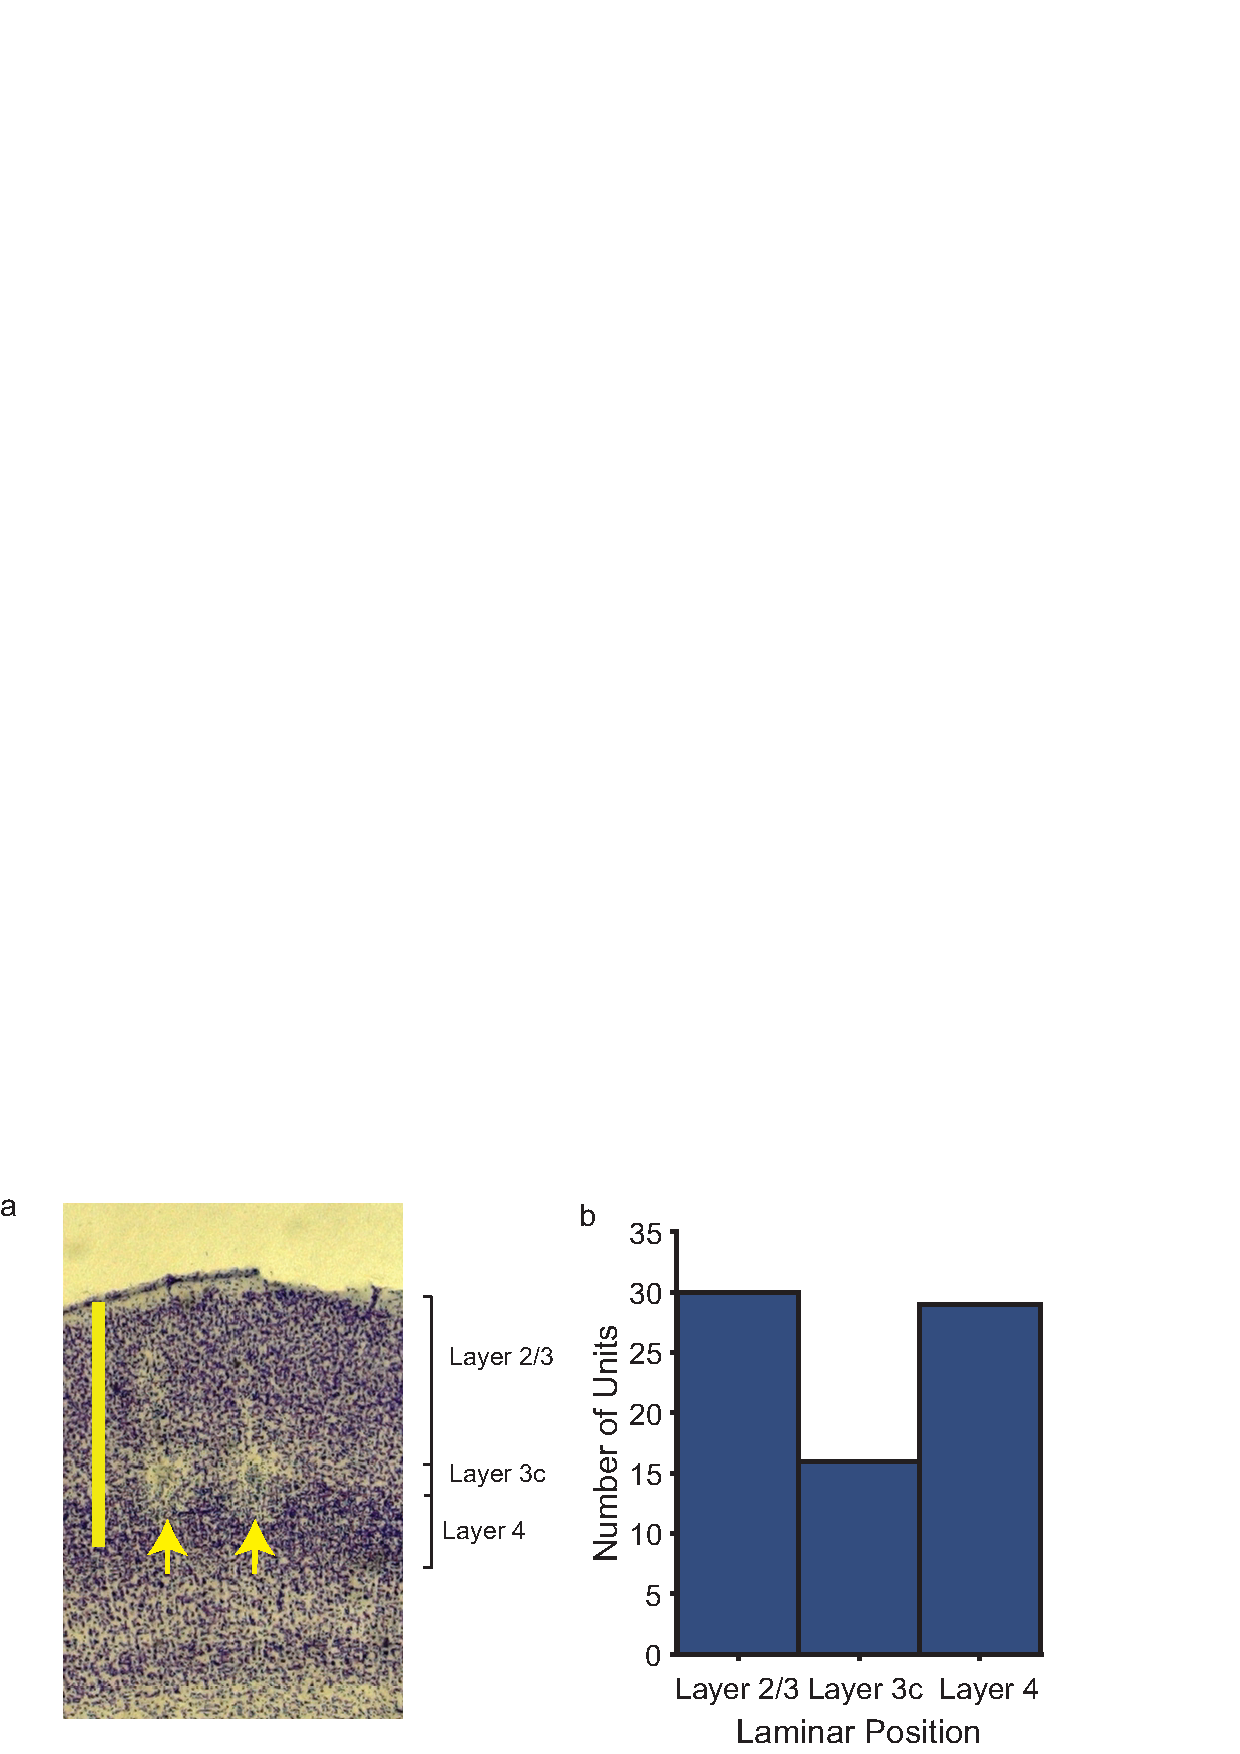
\includegraphics[width=\linewidth]{ShrewV1/LaminarPosition.jpg}
	\caption{The distribution of laminar positions from which we recorded. a) A photomicrograph of the tree shrew primary visual cortex with layers 2/3, 3c and 4 marked. The two arrows point to two lesions made in layer 3c of two separate tracks. The scale bar is 1 mm. b) Histogram showing the number of neurons recorded from each of the layers.}
	\label{fig:lp}
\end{figure} 

\subsubsection{Distribution of the circular variance}

The distribution of circular variances for neurons in the three layers, calculated from their responses to thin moving bars are shown in fig \ref{fig:cv}. The median CV of layer 2/3 neurons was 0.59 (n=28; 95\% CI= [0.32, 0.68]) ; that of layer 3c was  0.87 (n= 16; 95\% CI=[0.68, 0.91]) and that of layer 4 was 0.88 (n=29; 95\% CI=[0.84, 0.90 ]). The three distributions were significantly different from each other (p$<$0.001, Kruskal-Wallis test). Post-hoc tests revealed that there was a statistically significant distribution between the distribution of CVs of neurons in layer 2/3 and layer 3c (Mann-Whitney U test, z=2.37; p$<$0.01) and between layer 2/3 and layer 4 (Mann-Whitney U test, z= 3.58, p$<$0.001). The difference between the distributions of CV of layer 3c neurons and layer 4 neurons was not statistically significant (Mann-Whitney U test, z= 0.67; p=0.25). 
	\begin{figure}[H]
	
	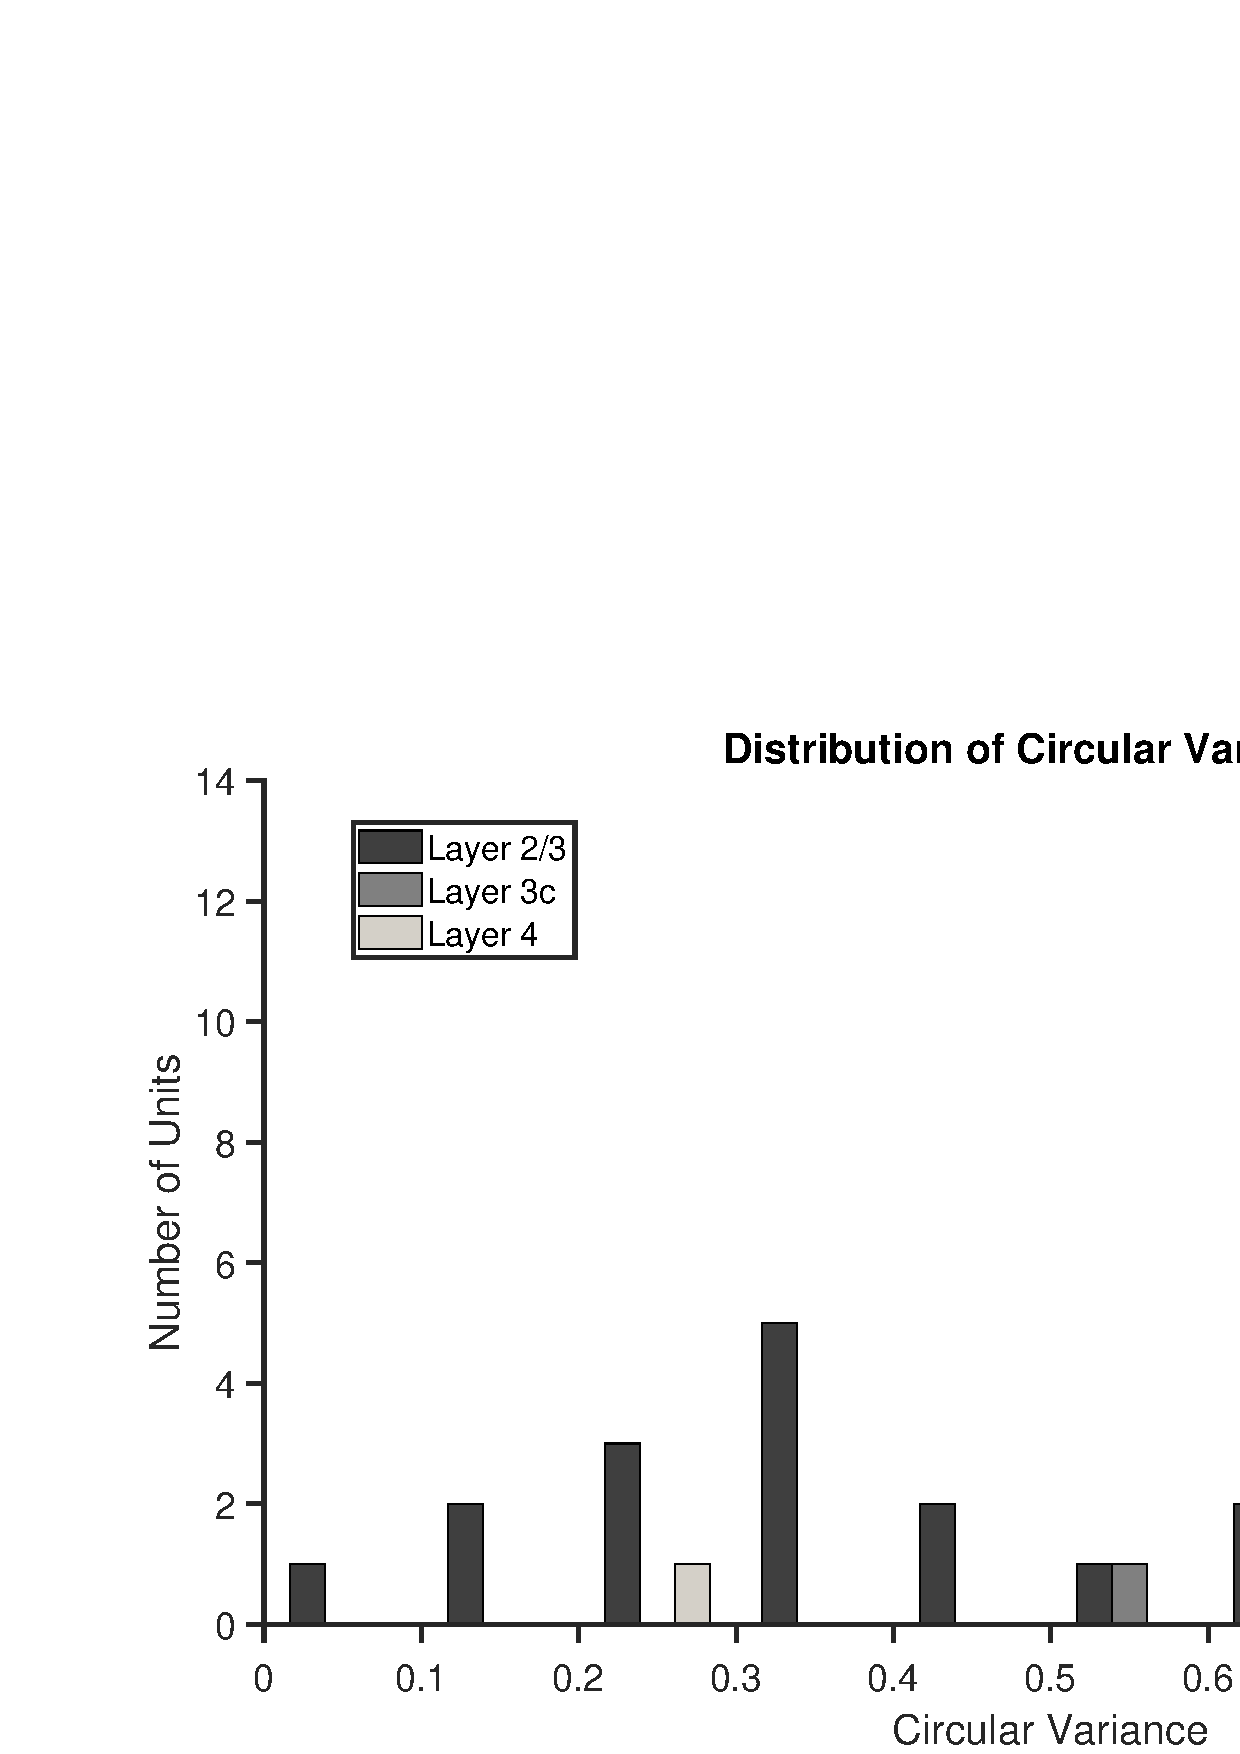
\includegraphics[width=\linewidth]{ShrewV1/cv_lamina_2_bw.jpg}
	\caption{The distribution of circular variance of neurons of the shrew V1.}
	\label{fig:cv}
\end{figure} 

\subsubsection{Circular mean of neurons}

According to our scheme of orientation selectivity in the tree shrews, layer 2/3 neurons inherit their orientation selectivity from layer 4 neurons which are biased for orientation. Here we test this hypothesis. Further, neurons in the tree shrew Layer 4 were thought to be untuned to orientation. However, recent studies, along with our own results in fig \ref{fig:cv} show that these neurons show orientation biases. Hence, we also wanted to determine if the orientation columns reported in the shrew Layer 2/3 extended to layer 4. As a result, we took the absolute difference between the circular means of each layer 2/3 neurons and subsequent neurons recorded from layers 3c and 4. These are shown in fig \ref{fig:cmdiff}.
	\begin{figure}[H]
	
	\includegraphics[width=\linewidth]{ShrewV1/cmdiff.jpg}
	\caption{The absolute difference between the circular mean of the first layer 2/3 neurons in each track and subsequent neurons from layer 3c and layer 4 in each track.}
	\label{fig:cmdiff}
	\end{figure}

Instead of the expected unimodal distribution where most neurons in a track were tuned to the same orientation, our results showed a bimodal distribution with approximately half the neurons tuned to the same orientation as the layer 2/3 neuron while the other half was tuned to an orientation that was 65$^o$ away.

We then split the distribution in two groups: pairs of neurons that were tuned to orientations less that 45$^o$ (group 1) apart and pairs tuned to orientation greater than 45$^o$ apart (Group 2). We then looked at whether the difference of was between the layer 2/3 neuron and layer 3c neurons or between layer 2/3 neuron and layer 4 neurons. These results are shown in fig \ref{fig:cmlayer}. We found that in group 1, the majority of the difference pairs were between layer 2/3 and layer 4 neurons (N=15; Binomial Distribution, p=0.04). In group 2, majority of the difference pairs were between layer 2/3 and layer 3c neurons (N=22; Binomial Distribution, p=0.04)

	\begin{figure}[H]
		
		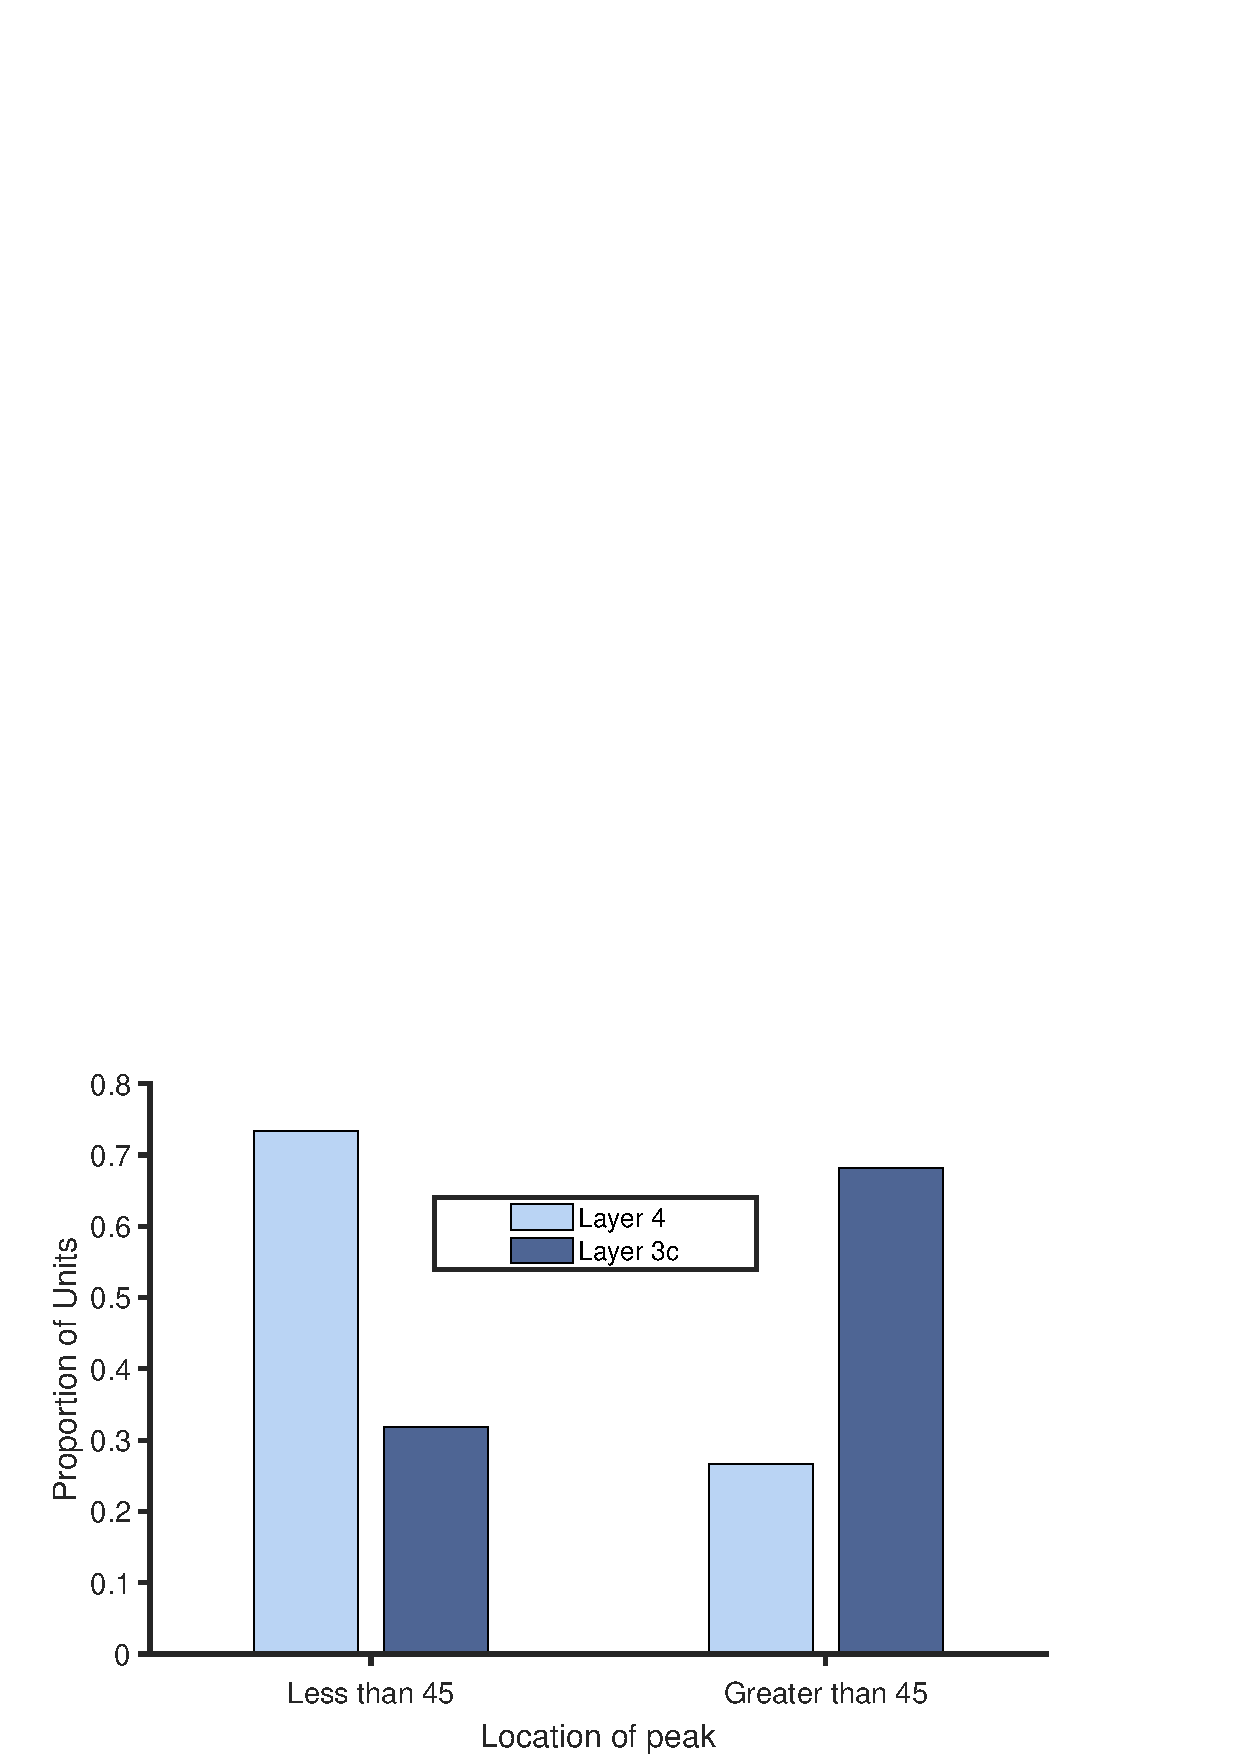
\includegraphics[width=\linewidth]{ShrewV1/cmlayer.jpg}
		\caption{The proportion of neurons from layers 3c and layer 4 with absolute differences greater and lesser than 45$^o$.}
		\label{fig:cmlayer}
	\end{figure}

In order to ensure that the second peak we observed in fig \ref{fig:cmdiff} wasn't due to track angles, we undertook a simulation experiment (see Methods, Random Simulation). We found that for the shortest distance between the layer 2/3 and layer 4 neurons in our sample (50 mm), there was a high probability of getting an absolute difference of 0 but this probability decreased steadily. For the greatest distance in our sample (300 mm), the probability of obtaining the same orientation diminished significantly. While there was a general trend towards getting neurons that were tuned 90$^o$ apart but there was no specific bias for a difference of 65$^o$. The highest probability of obtaining a peak at 65$^o$ was when distance was set at 250 mm (p=0.045).
		\begin{figure}[H]
		
		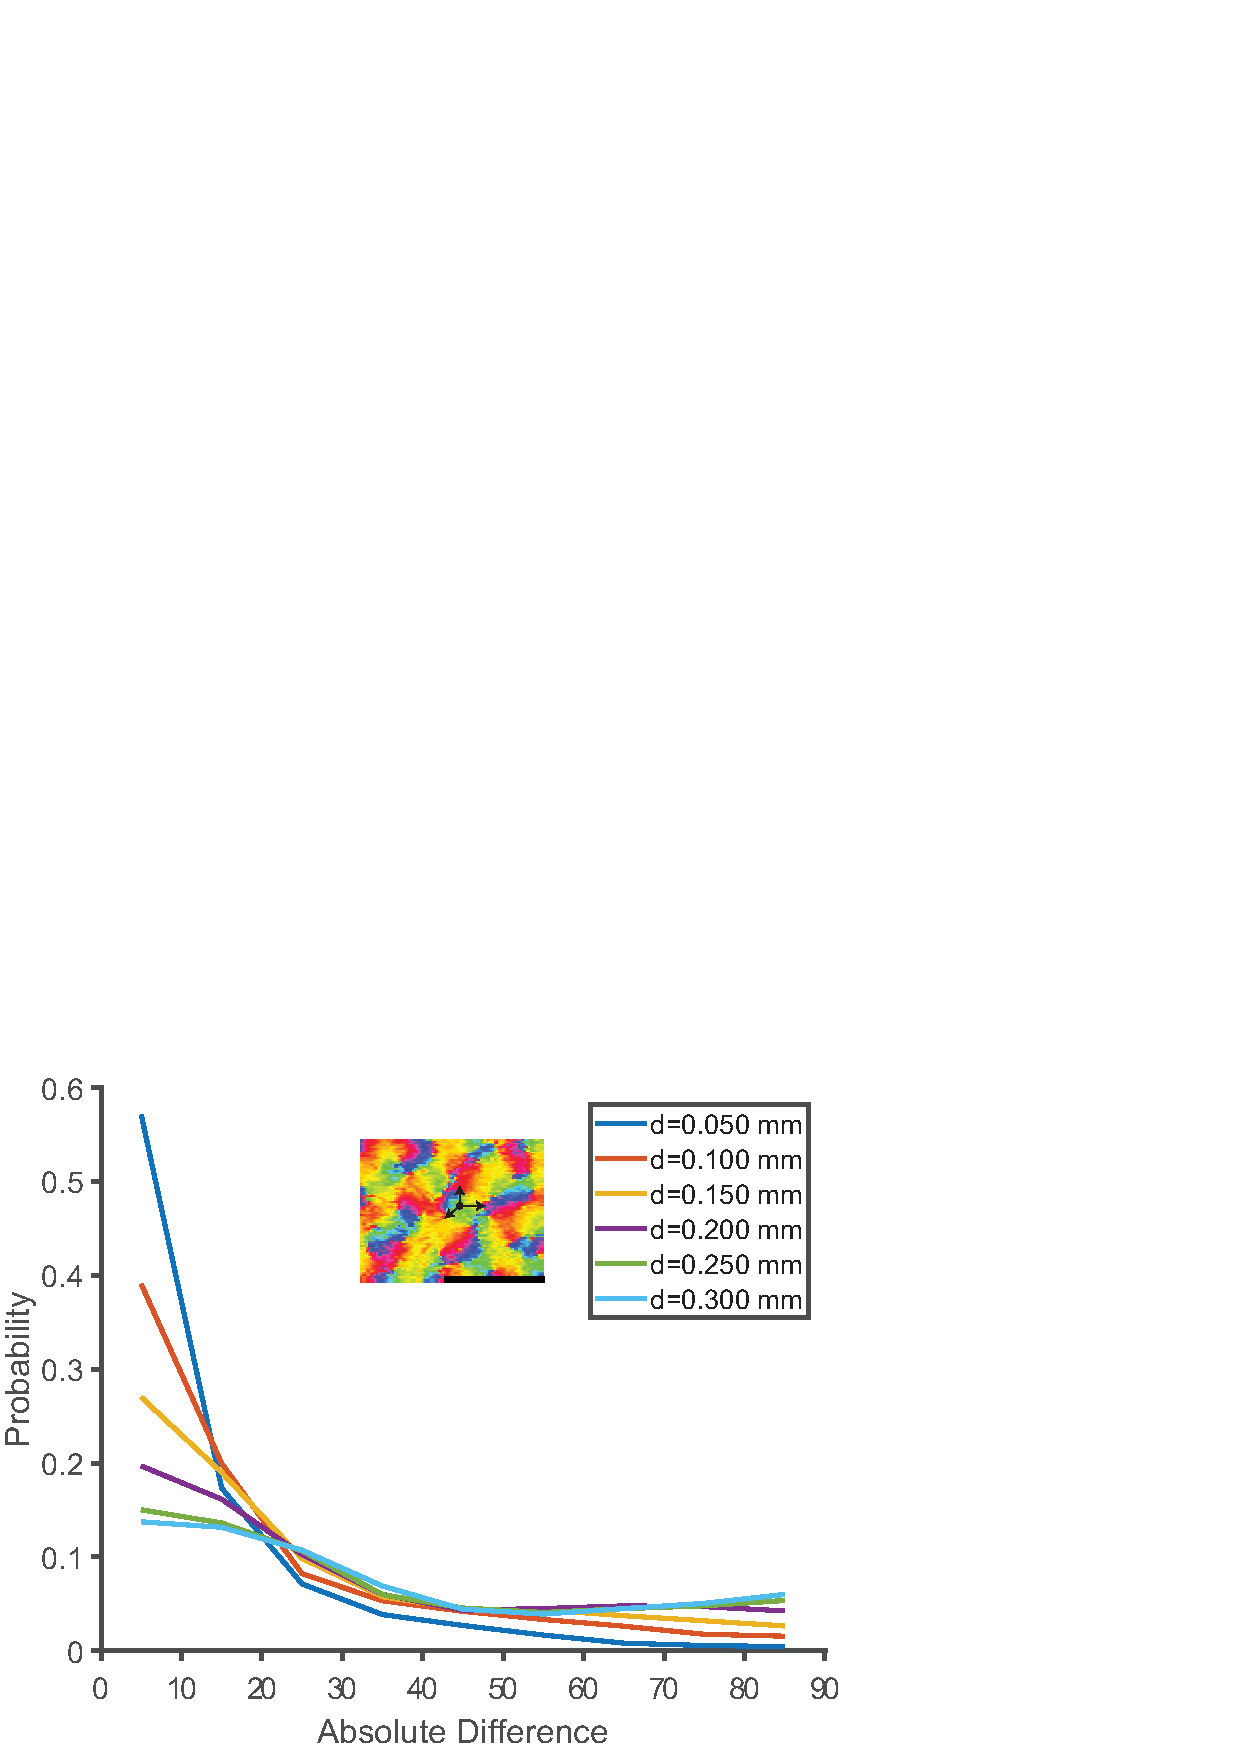
\includegraphics[width=\linewidth]{ShrewV1/simulation.jpg}
		\caption{Results of a simulation experiment: The orientation tuning map (inset) was taken from Bosking et al., 1997. On this map, points were randomly placed and the orientation of 1000 pixels randomly selected at one of the distances in the legend was subtracted from the original data point. For each distance, the distribution of absolute differences for the 1000 pixels are shown by the lines in the graph. Black line is 1mm.}
		\label{fig:sim}
	\end{figure}

\subsubsection{Spatial Frequency Tuning of neurons}

The distribution of the low cut-off, preferred and high cut-off spatial frequencies of the neurons in layer 2/3 and layer 4are shown in fig \ref{fig:sftuning}. Results from only these two layers are shown as we propose that the orientation selectivity of layer 2/3 neurons arise predominantly from layer 4 neurons. We found no significant differences between the spatial frequency tuning between the two layers, although layer 2/3 neurons show high spatial frequency attenuation. When the bandwidth of spatial frequency tuning in octaves was calculated, we found that the layer 2/3 neurons showed slightly sharper tuning (Median layer 2/3 b$_{oct}$= 2.2; n=16; Median layer 4 b$_{oct}$=2.3; n=9). This difference was however not statistically significant (Mann-Whitney U test; z=-1.18; p=0.24).

		\begin{figure}[H]
		
		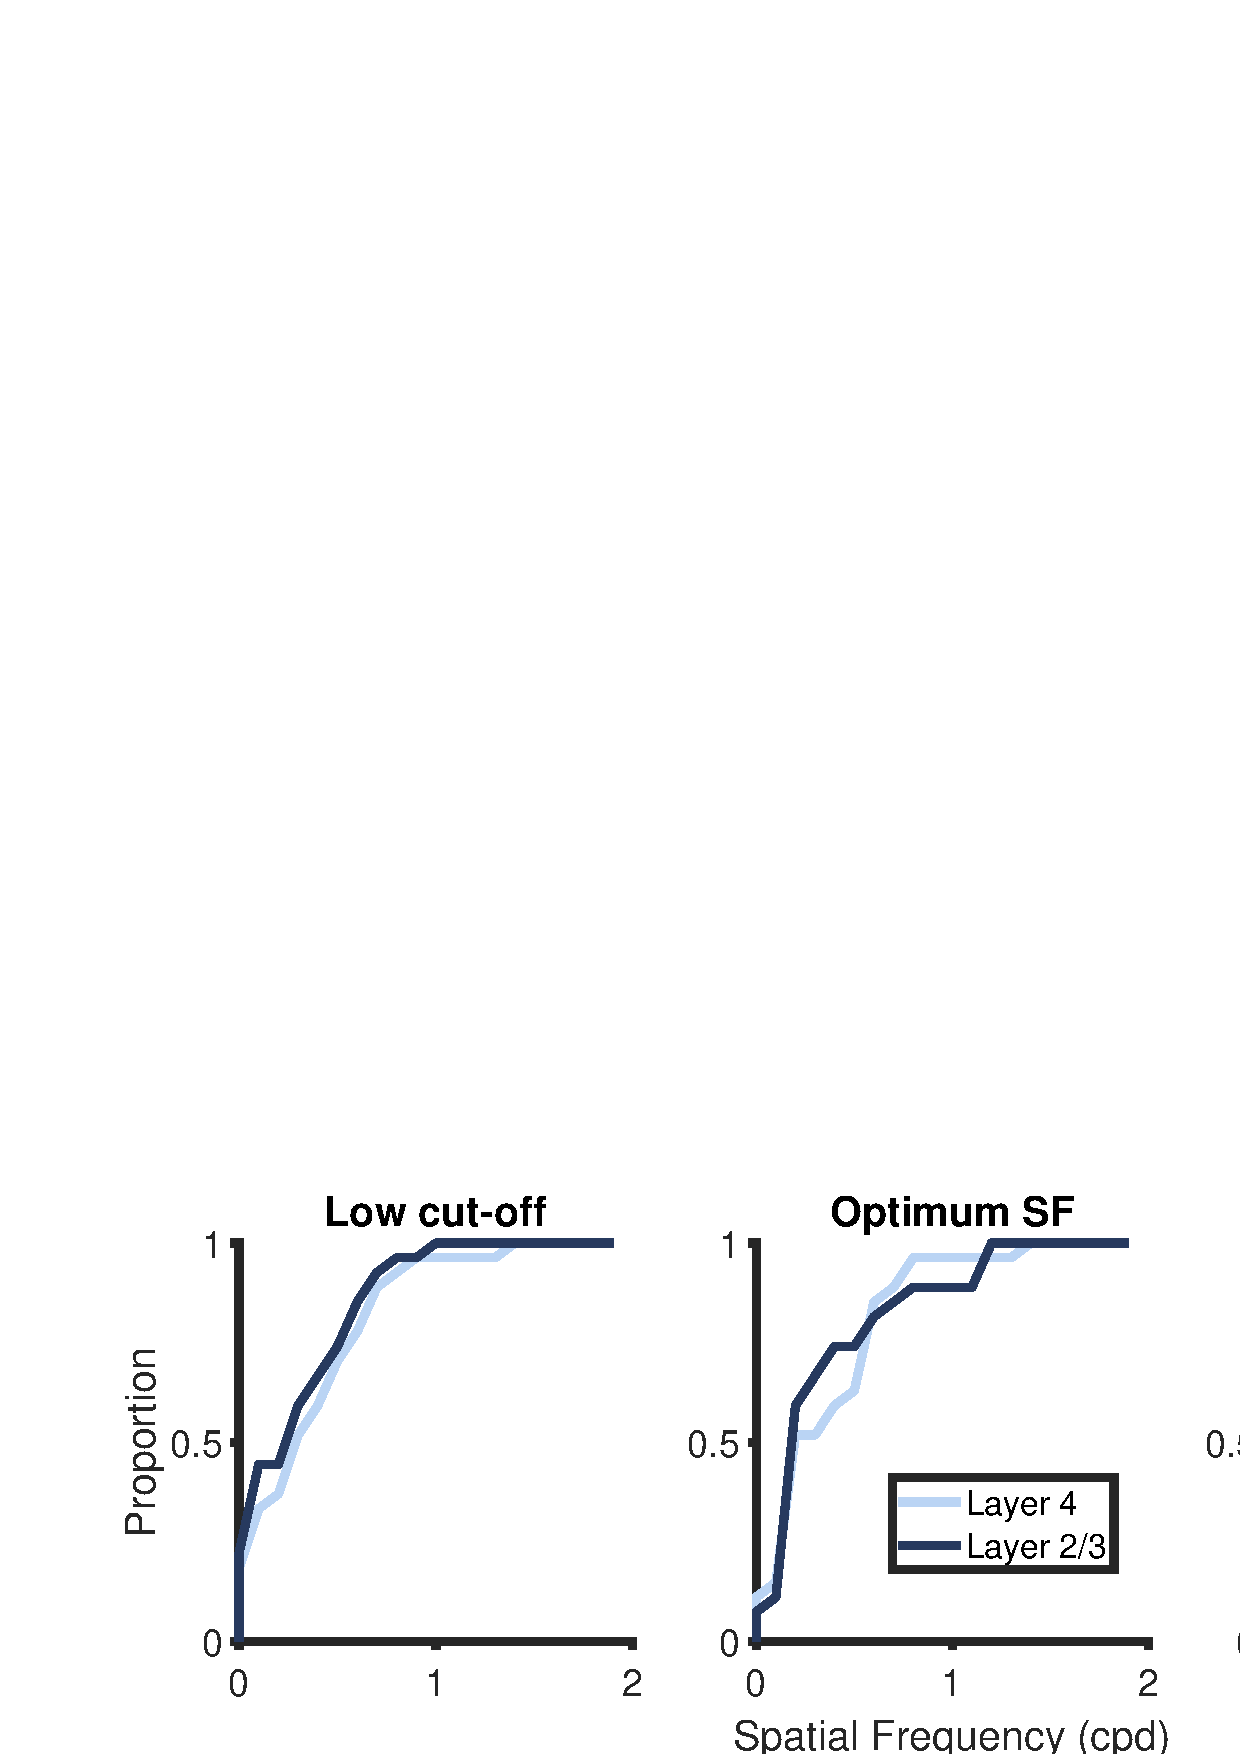
\includegraphics[width=\linewidth]{ShrewV1/sftuning_neurons_2.jpg}
		\caption{The cumulative distribution of the spatial frequency tuning of neurons in layers 2/3, 3c and 4 of the Shrew V1.}
		\label{fig:sftuning}
	\end{figure}

In our second hypothesis, we predicted that the layer 4 neurons will be more tuned to orientation at higher spatial frequencies. We tested this hypothesis by comparing the optimum spatial frequency tuning of layer 4 neurons with the spatial frequency where they demonstrated most orientation tuning in 20 neurons. These results are presented in figure \ref{fig:OSI4}. We can see that most neurons are located above the identity line, indicating that the spatial frequency where they are maximally tuned for orietnation is greater than the optimum spatial frequency of the neuron. The median optimum spatial frequency of the layer 4 neurons was 0.35 cpd (95\% CI= [0.2, 0.6]). The median of the spatial frequency where the orientation selectivity index was the highest was 0.8 cpd (95\% CI=[0.6, 1.2]). The spatial frequency at which the layer 4 neurons were most tuned for orientation was significantly higher than the neurons' optimum spatial frequency (Wilcoxon rank sum test, n=20, z= -2.93, p$<$0.005).


\begin{figure}[H]
	
	\includegraphics[width=\linewidth]{ShrewV1/layer4OSI_highres.jpg}
	\caption{The relationship between the optimum spatial frequency of the layer 4 neurons and the spatial frequency at which the layer 4 showed the highest OSI. The dashed line is the identity line. The solid red line is the result of a linear fit of the form y=mx+c to the data (m= 0.73 [-0.15, 1.61] and c=0.58 [0.15, 1.01]). }
	\label{fig:OSI4}
\end{figure}

In 18 individual tracks, we compared the spatial frequency and orientation tuning of the layer 2/3 neuron to that of the first layer 4 neuron we encountered. The results of this analysis is shown in fig \ref{fig:sfsum}. The result from an example neuron is shown in parts a and b. Fig \ref{fig:sfsum}a shows the spatial frequency tuning curve of layer 2/3 neuron and that of the corresponding layer 4 neuron to optimum and orthogonal orientation. We expected that the optimum spatial frequency of the layer 2/3 neuron and the spatial frequency at which the layer 4 neurons was most tuned for orientation would be similar. We found that this relation held true only in 3 of our 18 tracks. The median of the optimum spatial frequencies of the layer 2/3 neurons was 0.2 cpd (95\% CI= [0.1, 0.4]). In this sample of layer 4 neurons, the spatial frequency where the neurons were most tuned to orientation was 0.8 cpd (95\% CI=[0.3, 1.2]). In most of the tracks the maximum OSI of the layer 4 neuron occured at much higher spatial frequencies when compared to the optimum spatial frequency of the layer 2/3 neuron as demonstrated by the data points skewed closer to the y-axis (Wilcoxon signed rank test, n=18, p$<$0.005).
	\begin{figure}[H]
	
		\includegraphics[width=\linewidth]{ShrewV1/sfsummary.jpg}
		\caption{The cumulative distribution of the spatial frequency tuning of neurons in layers 2/3, 3c and 4 of the Shrew V1.}
		\label{fig:sfsum}
	\end{figure}

\section{Discussion}

In this chapter we set out to test if the orientation tuning of layer 2/3 neurons in the tree shrew primary visual cortex could arise by the sharpening of orientation biased inputs from layer 4 using non-specific inhibition. As we hypothesised, the orientation selectivity of the layer 4 neurons sharpened at higher spatial frequencies. We also found that the orientation selectivity of the layer 4 neuron and the corresponding layer 2/3 neurons were similar, however, the neurons in layer 3c of the same track seemed to be tuned to an orientation ~65$^o$ away. Finally, we hypothesised that the layer 2/3 neuron's peak sf would be similar to the spatial frequency where the layer 4 neuron showed maximum orientation tuning. We found that this was only true in a small proportion of the neuron pairs in our sample. In a majority of the pairs, the layer 4 neuron was optimally tuned at spatial frequencies higher than the optimum spatial frequency of the neurons. These results are further discussed below.


\paragraph{Distribution of orientation selectivity}

In this chapter we determined the orientation selectivity using bars for 73 V1 neurons from Layers 2/3, 3c and 4. We found that most neurons in layer 4 and layer 3c were broadly tuned for orientation. The broad orientation selectivity measured in the layer 4 is also consistent with this layer being similar to the LGN neurons when it comes to orientation selectivity (Reference). Layer 2/3 neurons show a bimodal distribution of orientation tuning when tested using bars with one group of neurons tuned quite sharply to orientation and another group tuned fairly broadly to orientation. There were no further sub-laminar differences in the distribution of this orientation selectivity within layer 2/3. These results are consistent with those reported earlier in the tree shrews (Van Hooser et al., 2013). 

Our results in layers 2/3 of the tree shrews are also consistent with those reported earlier in cats and macaques, where neurons in the primary visual cortex show a wide variety of orientation selectivities regardless of the layer. It should however be noted that neurons in layer 4 of the cats already show fairly sharp orientation selectivity and in layer 4C$\alpha$ of macaques too there are neurons that show sharp orientation selectivity. However neurons in layer 4C$\beta$ show broad orientation selectivity and regardless of the median orientation selectivity, neurons in all layers showed a wide range of orientation selectivity, especially as reported in layer 2/3 here (Ringach et al., 2002 etc).

\paragraph{Orientation selectivity of layer 3c neurons}

In our sample, we found that the neurons of layer 3c in the shrew V1 were broadly tuned to orientation despite being in the supragranular layers. These results are similar to those reported by Van Hooser and colleagues. In an earlier paper, it was shown that neurons in top and bottom parts of layer 4 projected to layer 3c (Fitzpatrick, 1996). The layer 4 neurons that project to the layer 3c neurons show sharper orientation tuning when compared to that of the layer 3c neurons. However, it makes no sense to develop orientation selectivity only to loose it at the very next step of processing. An alternate explanation could be that the broad orientation selectivity we see in the layer 3c is due to neurons in this layer receiving direct LGN inputs from layer 2(?), which is meant to have W-like cells. Similarly the layer 3C analogue in the macaques, layer 3B neurons which receive strong koniocellular inputs also show broad orientation tuning.

Another possibility could be that the neurons in layer 3c could be providing inhibitory inputs to the layer 2/3 neurons. The optimum orientation of the neuron was often 65$^o$ away from the orientation of the layer 2/3 neuron. In our scheme, layer 2/3 neurons sharpen the orientation biases from the layer 4 neurons by disynaptic inhibitory inputs from neurons tuned to orthogonal orientations. Anatomically, these inputs could be provided by the extensive horizontal connections in layer 2/3. However, having neurons tuned to the orthogonal or near orthogonal orientation organised in layers could provide an economy of connections that the long range horizontal inputs could not provide. In line with this, it has been shown that layer 3c does not have any significant horizontal connections and project upwards into layer 2/3, indicating that these neurons could be the source of the unoriented or orthogonally oriented disynaptic inhibitory inputs.

\paragraph {Spatial Frequency Dependence of Orientation Tuning in layer 4 neurons}

When we examined to see if the orientation selectivity of layer 4 neurons varied in relation to the spatial frequency tuning of the neurons, we found that in most cases, layer 4 neurons showed sharper orientation selectivity at higher spatial frequencies. This sharpening at high spatial frequencies has been previously reported in the retina and LGN of cats (Hammond, 1974; Levick and Thibos, 1980, 1982; Vidyasagar and Urbas, 1982) and macaques (Passaglia et al., 2002; Smith et al., 1990). This indicates that the sharpening of orientation selectivity observed from the layer 4 to layer 2/3 neurons in this case might employ a similar mechanism to that in cats---from LGN to layer 4--- and in macaques --- from Magnocellular layers in LGN to layer 4C$\alpha$. We also found that in some cases, the orientation selectivity of the neuron was higher at lower spatial frequencies. We are unsure what this is about.


\paragraph{Distribution of Spatial Frequency}

We examined the difference in the spatial frequency tuning between layer 2/3 neurons and layer 4 neurons. According to our scheme, if layer 2/3 neurons got their orientation selectivity from layer 4 neurons, then, a higher proportion of layer 2/3 neurons will show bandpass spatial frequency tuning when compared to layer 4 neurons. However, we found that there was no significant difference in the proportion of band pass tuned neurons between layer 4 and layer 2/3. These results are contradictory to those reported in by Van Hooser et al., 2013. One sigificant difference between our studies is the method used to estimate the spatial frequency tuning. They used a difference of gaussian curve to get the low cut-off, peak and high-cutoff spatial frequencies of the neurons. This method assumes that neurons have center-surround organisation as has been shown in the retinal ganglion and LGN neurons. Mathematically, they also did not use a separate term for the peak spatial frequency which means that the fit would only show a band-pass spatial frequency tuning if the peak spatial frequency was significantly greater than 0 cpd. We found that a significant proportion of neurons in our sample had fairly low optimum spatial frequencies which  may have been classified as low pass tuning using the DOG method whereas were classified as band-pass tuned using our method. We also found that there was a small degree of high spatial frequency attenuation in the neurons. This could be due to the small increase in receptive field sizes from layer 4 to layer 2/3 which reduces acuity. This high spatial frequency attenuation also explains the narrower tuning bandwidths of layer 2/3 neurons.

We also hypothesised that the peak spatial frequency of the layer 2/3 neurons would be similar to the spatial frequency where the orientation tuning of the layer 4 neuron was greatest. However, we found this in only a small proportion of the neurons in our study. For this to be the case in a majority of the studies, layer 2/3 neurons needed to have higher peak spatial frequencies when compared to the layer 4 neurons. However, there hasn't been any systematic overrepresentation of higher spatial frequencies in the layer 2/3 neurons in our study. Several studies in the past have suggested that neurons in the V1 of cats and macaques may be organised in columns, similar to that seen in orientation selectivity. We didn't find any such consistency either. There seems to be a continuous distribution of most spatial frequencies in the cortex. As a result, within a single track, there could be several neurons all tuned to different spatial frequencies projecting the layer 2/3 neurons. As a result, for this hypothesis to be tested correctly, we would need to undertake simultaneous recordings from the layer 2/3 and layer 4 neurons and record from pairs that are connected. Despite these caveats, we found our expected results in 3 pairs of neurons with a few other pairs bunched close to the identity line. As a result, while we cannot definitely conclude that neurons in layer 2/3 use non-specific inhibition to sharpen the orientation biases inherited from the layer 4 neurons, we do have some evidence that suggests that this could be the mechanism through which orientation arises in some neurons in the tree shrew V1. 

